  \documentclass[lnbip]{svmultln}

\usepackage[T1]{fontenc}
\usepackage[utf8]{inputenc}
\usepackage{ragged2e}
\usepackage[bookmarks=false,colorlinks,urlcolor=blue,%
linkcolor=magenta,citecolor=red,linktocpage=true,breaklinks=true]{hyperref}
\usepackage{cleveref}
\usepackage{xspace}
\usepackage{graphics}
\usepackage{inconsolata}
\usepackage{xcolor}
\usepackage{fancyvrb}
\usepackage{listings}
\lstset{escapeinside={<@}{@>}}
\usepackage{xparse}
\usepackage{tikz}
\usetikzlibrary{arrows}
\usepackage{pgf-umlsd}
 
% \linespread{.97}
% \usepackage[backend=bibtex,style=ieee,giveninits,maxnames=2,minnames=1]
% {biblatex}

% \AtEveryBibitem{\clearfield{pages}}
% \AtEveryBibitem{\clearfield{volume}}
% \AtEveryBibitem{\clearfield{number}}
% \addbibresource{biblio.bib}

\usepackage{bold-extra}

\newcommand{\Jolie}{Jolie}
\newcommand{\Definition}{\noindent\textbf{\emph{Definition}}}
\newcommand{\Implementation}{\noindent\textbf{\emph{Implementation}}}
\newcommand{\Section}{\S}

\newcommand{\citeNeed}{{\color{red}[CitNeed]}}

\definecolor{color:keyword}{rgb}{0.53,0.05,0.05}
\definecolor{color:comment}{rgb}{0.25,0.37,0.75}
\definecolor{color:string}{rgb}{0.87,0.0,0.0}

\lstdefinelanguage{Jolie}{
	morekeywords={csets,type,raw,any,undefined,void,default,if,for,while,spawn,foreach,else,define,main,include,constants,inputPort,outputPort,interface,execution,cset,nullProcess,RequestResponse,OneWay,throw,throws,install,scope,embedded,init,synchronized,global,is_defined,is_int,is_bool,is_long,is_string,bool,long,int,string,double,undef,with,Location,Protocol,Interfaces,Aggregates,Redirects,linkIn,linkOut},
	sensitive=true,
	morecomment=[l]{//},
	morecomment=[s]{/*}{*/},
	morestring=[b]",
	otherkeywords={;,|,@}
}

\lstset{
	language=Jolie,
	mathescape=true,
	resetmargins=true,
	numberstyle=\footnotesize,
	numbers=left,
	numbersep=5pt,
	numberblanklines=true,
	basicstyle=\ttfamily\small,
	tabsize=2,
	%frame=lines,
	commentstyle=\ttfamily\color{color:comment},
	stringstyle=\color{color:string},
	captionpos=b,
	keywordstyle=\bfseries\color{color:keyword},
	showstringspaces=false,
	belowcaptionskip=10mm,
	breaklines=false,
	columns=fullflexible,
	linewidth= 0.8\linewidth
}


\colorlet{punct}{red!60!black}
\definecolor{delim}{RGB}{20,105,176}
\definecolor{keyword}{RGB}{48,0,211}
\colorlet{numb}{magenta!60!black}

\newcommand{\kwd}[1]{{\color{keyword}\textbf{#1}}}
\newcommand{\hid}[1]{{\color{gray}#1}}

\lstdefinelanguage{json}{
    basicstyle=\ttfamily\small,
    commentstyle=\color{color:comment}, % style of comment
    stringstyle=\color{color:string}, % style of strings
    numbers=left,
    numberstyle=\scriptsize,
    stepnumber=1,
    numbersep=8pt,
    showstringspaces=false,
    frame=lines,
    string=[s]{"}{"},
    comment=[l]{:\ "},
    morecomment=[l]{:"},
    literate=
        *{0}{{{\color{numb}0}}}{1}
         {1}{{{\color{numb}1}}}{1}
         {2}{{{\color{numb}2}}}{1}
         {3}{{{\color{numb}3}}}{1}
         {4}{{{\color{numb}4}}}{1}
         {5}{{{\color{numb}5}}}{1}
         {6}{{{\color{numb}6}}}{1}
         {7}{{{\color{numb}7}}}{1}
         {8}{{{\color{numb}8}}}{1}
         {9}{{{\color{numb}9}}}{1}
}

\newcommand{\code}[1]{\lstinline{#1}{}}

\newcommand{\setUmlSeqChartStyle}{
	\tikzset{inststyle/.style={
    rectangle, draw, 
    anchor=west, 
    minimum height=0.8cm, 
    minimum width=1.6cm, 
    fill=white
    %drop shadow={opacity=0,fill=black}]
    }
  }
}

\crefname{figure}{Fig.}{Figs.}
\crefname{lstlisting}{Listing}{Listings}
\newcommand*\circled[1]{\tikz[baseline=(char.base)]{
            \node[shape=circle,draw,inner sep=1.3pt] (char) {#1};}}


\usepackage[textsize=tiny,linecolor=teal,%
bordercolor=teal,backgroundcolor=lime!25]{todonotes} % for margin
\setlength{\marginparwidth}{2cm}

\begin{document}

\mainmatter              % start of the contribution

\title{Linguistic Abstractions for\\ Interoperability of IoT Platforms}

\titlerunning{Language Abstractions for Interoperability of IoT
Platforms}  % abbreviated title (for running head)

\author{Maurizio Gabbrielli\inst{1} \and 
Saverio Giallorenzo\inst{2} \and 
Ivan Lanese\inst{1} \and Stefano Pio
Zingaro \inst{1}}
%
\authorrunning{Gabbrielli M. et al.}   % abbreviated author list (for
% running head)
%
%%%% list of authors for the TOC (use if author list has to be modified)
\tocauthor{Maurizio Gabbrielli, Saverio Giallorenzo, Ivan Lanese, Stefano Pio
Zingaro}
%
\institute{Universit\`a di Bologna / INRIA \\
\and
University of Southern Denmark}

\maketitle

% The Internet of Things (IoT) promotes the communication among
% heterogeneous entities, from small sensors to Cloud systems. However,
% this is realized using a wide range of communication media and data
% protocols, usually incompatible with each other. Thus, IoT systems
% tend to grow as homogeneous isolated platforms, which hardly
% interact. In this paper we propose a language-based approach for
% communication technology integration to achieve a higher degree of
% interoperability among disparate IoT platforms. We build on the Jolie
% programming language, which provides uniform linguistic abstractions
% to exploit heterogeneous communication stacks, allowing the programmer
% to specify in a declarative way the desired stack, and to easily
% change it, even at runtime.  Jolie currently supports the main
% technologies from Service-Oriented Computing, such as TCP/IP,
% Bluetooth, and RMI at transport level, and HTTP and SOAP at
% application level. We integrate in Jolie the two most adopted
% protocols for IoT communication, i.e., CoAP and MQTT. We report our
% experience, including a case study in the home automation area, and we
% present high-level concepts valuable both for the general
% implementation of interoperable systems and for the development of
% other language-based solutions.

\begin{abstract}
The Internet of Things (IoT) advocates for multi-layered platforms---from edge
devices to Cloud nodes---where each layer adopts its own communication
standards (media and data formats). While this freedom is optimal for in-layer
communication, it puzzles cross-layer integration due to incompatibilities
among standards. Also enforcing a unique communication stack within the same
IoT platform is not a solution, as it leads to the current phenomenon of ``IoT
islands'', where disparate platforms hardly interact with each other. In this
paper we tackle the problem of IoT cross-layer and cross-platform integration
following a language-based approach. We build on the Jolie programming
language, which provides uniform linguistic abstractions to exploit
heterogeneous communication stacks, allowing the programmer to specify in a
declarative way the desired stack, and to easily change it, even at runtime.
Jolie currently supports the main technologies from Service-Oriented Computing,
such as TCP/IP, Bluetooth, and RMI at transport level, and HTTP and SOAP at
application level. We integrate in Jolie the two most adopted protocols for IoT
communication, i.e., CoAP and MQTT. We report our experience on a case study on
Cloud-based home automation, and we present high-level concepts valuable both
for the general implementation of interoperable systems and for the development
of other language-based solutions.
\end{abstract}

\section{Introduction}
\label{sec:intro}
The Internet of Things (IoT) advocates for multi-layered software platforms,
each adopting its own media protocols and data
formats~\cite{GubbiBMP13,Atzori20102787,7123563}.
%
The problem of integrating layers of the same IoT platform, as well as
different IoT vertical solutions, involves many levels of the communication
stack, spanning from link-layer communication technologies, such as ZigBee and
WiFi, to application-layer protocols like HTTP,
CoAP~\cite{coap,doi:10.17487/RFC7252}, and MQTT~\cite{mqtt,mqtt-v3.1.1},
reaching the top-most layers of data-format
integration~\cite{Milenkovic:2015:CII:2843962.2822643}.

Technology-wise, architects of IoT platforms can choose between two approaches
at odds. The first approach favors optimal in-layer communications, i.e.,
choosing media protocols and data formats best suited for the interactions
happening among homogeneous elements, e.g., edge devices (connectionless
protocols and binary data formats~\cite{7123563}), mid-tier controllers
(gateways and aggregators on the RESTful stack~\cite{richardson2008restful}),
or Cloud nodes (scalable publish-subscribe message
queues~\cite{garg2013apache}). Following this first approach
is optimal for in-layer communication. However, at the cross-layer level, the heterogeneity
and possible incompatibility of the chosen standards make enforcing integrity
within the IoT system complex and the resulting integration fragile. The second architectural approach
favors cross-layer consistency, enforcing a unique communication stack over a
single IoT platform. Here cross-layer integration is simpler thanks to the
adoption of a single medium and data format. However such enforced uniformity is
the main cause of the phenomenon known as ``IoT
island''~\cite{Soursos16,Gojmerac16}, where IoT platforms take the shape of
vertical solutions that provide little support for collaboration and
integration with each other. How to overcome this limitation is currently a hot
topic, tackled also by ongoing EU projects, e.g., symbIoTe~\cite{Gojmerac16}
and bIoTope~\cite{biotope}.

In this paper we tackle the problem of IoT integration (both cross-layer and
cross-platform) following a language-based approach focused on integration at
both the transport (TCP or UDP) and application layer. To reach our goal we do
not start from scratch, but we leverage the work done in the area of
Service-Oriented Architectures (SOAs)~\cite{Erl07} and we build on the Jolie
programming language~\cite{MONTESI200719,MGZ07,MontesiGZ14,jolie-lang}. In
particular, we rely on those abstractions provided by Jolie that \emph{i}) let
different communication protocols seamlessly coexist and interoperate within
the same program and \emph{ii}) let programmers dynamically choose which
communication stack should be used for any given communication.
%
Concretely, we fork the Jolie interpreter---written in Java---into a prototype
called JIoT~\cite{jiot}, standing for ``Jolie for IoT''.
%
JIoT supports all the protocols already supported by the Jolie interpreter (TCP at the transport level, and protocols such as SOAP, RMI and HTTP at the application level), while adding the application-level protocols for IoT, namely CoAP (and, as a consequence, UDP at the transport level) and MQTT.
Notably, when the application protocol supports different
representation formats (such as JSON, XML, etc.) of the message payload, as in
the case of HTTP and CoAP, JIoT, like Jolie, can automatically marshal and un-marshal data
as required.

We structure our presentation as follows. We overview in \cref{sec:approach}
our approach and summarize our contribution in \cref{sec:contribution}. Then,
we discuss the main challenges we faced in our development in
\cref{sec:challenges}, we present how a programmer can use CoAP/UDP
(\cref{sub:coap}) and MQTT (\cref{sub:mqtt}) in JIoT, and we detail our
implementation in \cref{sub:implementation}. We describe, in \cref{sub:case},
a scenario on Cloud-based home automation where a JIoT architecture
coordinates heterogeneous edge devices. Finally, we position our contribution
with respect to related work in \cref{sec:related} and we draw final remarks
in \cref{conclusion}.

JIoT is available at~\cite{jiot}, released under the LGPL v2.1 license. The
code snippets reported in this paper are based on version 1.2 of JIoT. The
integration of JIoT into the official code-base of the Jolie language is
ongoing work.

\section{Approach Overview}
\label{sec:approach}

Without proper language abstractions, guaranteeing interoperability among
protocols belonging to different technology stacks is highly complex. The
problem is further exacerbated when one has to modify the technology stack used
for some specific interaction. The replacement may be either static, e.g.,
because of the deployment of new, heterogeneous devices in a pre-existing
system, or dynamic, e.g., to support a changing topology of disparate mobile
devices. Contrarily, with JIoT most of the complexity of guaranteeing
interoperability is managed by the language interpreter and hidden from the
programmer.

As an illustrative example of the proposed approach, let us consider a scenario
where we want to integrate two islands of IoT devices, both collecting
temperature data, but relying on different communication stacks, namely HTTP
over TCP and CoAP over UDP.
%
The end goal is to program a collector which receives and aggregates
temperature measurements from both islands.

Following the structure of Jolie programs, the collector programmed in JIoT is
composed of two parts: a \emph{behavior}, specifying the logic of the
elaboration, and a \emph{deployment}, describing in a declarative way how
communication is performed. This separation of concerns is fundamental to let
programmers easily change which communication stack to use, preserving the same
logic for the elaboration.

As an example of program behavior, let us consider the code below, where \lstinline{main} is the entry point of execution of Jolie programs.
%
\begin{lstlisting}[numbers=left,basicstyle=\footnotesize\ttfamily]
main {
  ...
  receiveTemperature( data );
  ...
}
\end{lstlisting}
%
Above, Line 3 contains a reception statement.
Receptions in Jolie indicate a
point where the program waits to receive a message.
In this case, the collector
waits to receive a temperature measurement on \emph{operation}
\code{receiveTemperature} (an operation in Jolie is an abstraction for
technology-specific concepts such as channels, resources, URLs,
\dots). Upon reception, it stores the retrieved value in variable \code{data}.
%
Besides the logic of computation of the collector, we also need to specify the deployment, i.e., on
which technologies the communication happens; in the example above, how the
collector receives messages from other devices. In Jolie this information is
defined within \emph{ports}. For example, the port to receive (denoted with
keyword \code{inputPort}) HTTP measurements can be defined as in \cref{lst:ex_port}.
%
\begin{figure}
\begin{lstlisting}[numbers=left,basicstyle=\ttfamily\footnotesize,caption=Example of interface
and input port in Jolie.,label=lst:ex_port]
interface TemperatureInterface {
 OneWay: receiveTemperature( string )
}

inputPort CollectorPort1 {
 Location: "socket://localhost:8000"
 Protocol: http
 Interfaces: TemperatureInterface
}
\end{lstlisting}
\end{figure}
%
Port \code{CollectorPort1} specifies that the collector expects inbound
communications via \code{Protocol} \code{http} using a TCP/IP socket receiving
at URL \code{"localhost"} on TCP port \code{8000}. A port exposes a set of operations, collected within a set of \code{Interfaces}. In the example, the input port \code{CollectorPort1} declares to expose interface \code{TemperatureInterface}, which is defined at lines 1--3 of Listing of \code{interface} is declared at lines 1--3 of \cref{lst:ex_port}. The interface declares the operation
\code{receiveTemperature}, including the type of expected data
(\code{string}), as a \code{OneWay} operation, namely an asynchronous
communication that does not require any reply from the collector (except the
acknowledgment automatically provided by the TCP implementation).

Thanks to port \code{CollectorPort1}, the collector can receive data from the
HTTP island. To integrate the second island, we just need to define an
additional port, similar to \code{CollectorPort1}, except for using UDP/IP
datagrams at the transport layer and CoAP~\cite{doi:10.17487/RFC7252,coap} at the application layer. Hence, the
whole code of the collector becomes:
%
\begin{lstlisting}[%
  basicstyle=\footnotesize\ttfamily,
  label=temperature_interface,
  caption=Code of the Collector Example.]
interface TemperatureInterface {
 OneWay: receiveTemperature( string )
}

inputPort CollectorPort1 {
 Location: "socket://localhost:8000"
 Protocol: http
 Interfaces: TemperatureInterface
}

inputPort CollectorPort2 {
 Location: "datagram://localhost:5683"
 Protocol: coap
 Interfaces: TemperatureInterface
}

main {
 ...
 receiveTemperature( data );
 ...
}
\end{lstlisting}
%
The example above highlights how, using the proposed language abstractions, the
programmer can write a unique behavior and exploit it to receive data sent over
heterogeneous technology stacks. Indeed, the \code{receiveTemperature}
operation takes measurements from both the \code{inputPort}s.
%
For instance, if communication over \code{Collector2} fails, port
\code{Collector1} can still receive data.
%
Programmers can also specify elaborations that depend on the used technologies,
by using different operations in different ports.
Jolie supports both inbound and outbound
communications, the latter declared with \code{outputPort}s, whose structure
follows that of \code{inputPort}s. Furthermore, the \code{Location} and
\code{Protocol} of \code{outputPort}s can be changed at runtime, enabling the
dynamic selection of the appropriate technologies for each context.

As mentioned, Jolie enforces a strict separation of concerns between behavior,
describing the logic of the application, and deployment, describing the
communication capabilities. The behavior is defined using the typical
constructs of structured sequential programming, communication primitives, and
operators to deal with concurrency (parallel composition and input
choices~\cite{MontesiGZ14}).

Jolie communication primitives comprise two modalities of interaction.

Outbound~\code{OneWay} communications send a message asynchronously, while
\code{RequestResponse} communications send a message and wait for a reply (they
capture the well-known pattern of request-response
interactions~\cite{req-rep}). Dually, inbound \code{OneWay} communications wait
to receive a message, without sending a reply, while inbound \code{RequestResponse}s wait for a message
and send back a reply.

%
Jolie supports many communication media (via keyword
\code{Location}) and data protocols (via keyword \code{Protocol}) in a simple,
uniform way. This is the main feature of the Jolie language, and the reason why
we base our approach on it.
%
Indeed, for each communication port the used medium and data protocol are
declared in the deployment part of the program.  In order to change the
used medium and protocol one just needs to change the declaration, without
affecting the behavior part which describes the actual computation.
Hence, functionalities defined by a single behavior can be made available using
different media and protocols by specifying different deployments. Being born
in the field of SOAs, Jolie supports the main communication media (TCP/IP
sockets, Bluetooth L2CAP, Java RMI, and Unix local sockets) and data protocols
(HTTP, JSON-RPC, XML-RPC, SOAP and their respective SSL versions) from this
area.

\section{Contribution}
\label{sec:contribution}
To substantiate the effectiveness of our language-based approach to IoT
integration, we add to Jolie support for the main communication stacks used in the
IoT setting. Concretely, the added contribution of JIoT with respect to Jolie
is the integration of two application protocols relevant in the IoT scenario,
namely CoAP~\cite{doi:10.17487/RFC7252,coap} and MQTT~\cite{mqtt-v3.1.1,mqtt}.
Notably, in JIoT the usage of such protocols is supported by the same
linguistic abstractions that Jolie uses for SOAs protocols such as HTTP and
SOAP.

Even if Jolie provides support for the integration of new protocols, when set
in the context of IoT technology, the task is non trivial. Indeed, all the
protocols previously supported by Jolie exploit the same internal interface,
based on two assumptions: \emph{i}) the usage of underlying technologies that
ensure reliable communications and \emph{ii}) a point-to-point communication
pattern.

However, both these assumptions fail when considering the two IoT technologies
we integrate:

\begin{itemize}
 \item CoAP communications can be unreliable since they are based on UDP
       connectionless datagrams. CoAP provides options for reliable communications,
       however these are usually disabled in an IoT setting, since battery and
       bandwidth preservation is important;

 \item MQTT communications are based on the publish-subscribe paradigm, which
       contrasts with the point-to-point communication found in Jolie primitives.
       Hence, we need to define a mapping of the general abstractions of the Jolie
       language onto the publish-subscribe paradigm, balancing two factors: \emph{i})
       preserving the simplicity of use of the point-to-point communication style and
       \emph{ii}) capturing the typical publish-subscribe flow of communications. Such
       a mapping is particularly challenging in the case of request-response
       communications. Remarkably, the mapping that we present in this work is general
       and could be used also in other contexts.
\end{itemize}

This paper integrates, revises, and extends material
from~\cite{GabbrielliGLZ18}, where we presented, discussed, and provided basic
technical details on the proposed language-based approach to IoT integration.
Main extensions comprise:

\begin{itemize}
 \item advanced technical details on our implementation (Section~\ref{sub:implementation}) including:

       \begin{itemize}
        \item a general account on how media and protocols are separated from the
              Jolie interpreter and how they can be developed as independent modules;

        \item extensive details on the implementation of UDP, CoAP, and MQTT
              protocols;

       \end{itemize}

 \item a comprehensive case study on a home automation scenario (Section~\ref{sub:case}) where we
       consider:

       \begin{itemize}

        \item local, cross-layer communication among edge devices and
              mid-tier controllers;

        \item remote, cross-layer interactions among Cloud nodes and mid-tier
              controllers.

       \end{itemize}

\end{itemize}
%
We conclude this section briefly discussing the current limitations of JIoT
related to its usage in the programming of low-level edge devices---like
Arduinos and other microcontrollers. JIoT supports dynamic scenarios where the
nodes in the network can switch among many technology stacks according to
internal or environmental conditions, such as available energy or quality of
communication. From preliminary discussions with collaborators and IoT
practitioners, we collected positive opinions on the idea of using JIoT for
programming low-level edge devices. Given these positive remarks, we
investigated the feasibility of running JIoT programs over edge devices,
possibly including additional language abstractions to provide low-level
access to in-board sensors and actuators. However, our survey revealed a
market of devices fragmented over incompatible hardware architectures and
characterized by strong constraints over both computational power and energy
consumption. Considering these limitations, we concluded that supporting the
execution of JIoT-like programs over edge devices would require a strong
engineering effort. While this research direction is promising, we deem it
non-urgent, since currently developers tend to program very simple behaviors
for edge devices~\cite{7123563}, which usually capture some data (e.g.,
through one of their sensors) and then send them to mid-to-top-tier devices.
The latter category of devices are often used to process and coordinate the
flow of data, having more powerful hardware, reliable communication channels,
and less constraints on energy consumption. Based on this considerations, in
this work we omit the low-level programming of edge devices and we focus on
mid-to-top-tier ones, which can host the JIoT runtime and whose topological
context benefits from the flexibility of the approach.


\section{JIoT: Jolie for IoT}
\label{sec:challenges}
Jolie currently supports some of the main technologies used in SOAs (e.g.,
HTTP, SOAP). However, only a limited amount of IoT devices uses the media and
protocols already supported by Jolie. Indeed, protocols such as
CoAP~\cite{doi:10.17487/RFC7252,coap} and MQTT~\cite{mqtt-v3.1.1,mqtt}, which
are widely used in IoT scenarios, are not implemented in Jolie. Integrating
these protocols, as we have done, is essential to allow Jolie programs to
directly interact with the majority of IoT devices. We note that emerging
frameworks for interoperability, such as the Web of Things~\cite{w3c17}, rely
on the same protocols we mentioned for IoT, thus JIoT is also compliant with
them.
%
However there are some
challenges linked to the integration of these technologies within Jolie:

\begin{itemize}
  \item \textit{lossless vs.\@ lossy protocols} --- In SOAs,
  machine-to-machine communication relies on lossless protocols: there are no
  strict constraints on energy consumption or bandwidth and it is not critical
  how many transport-layer messages are needed to ensure reliable delivery.
  That is not true in IoT networks, where communication is constrained by
  energy consumption, which defines what technology stack can be used. Indeed,
  many IoT communication technologies, among which the mostly renowned CoAP
  application protocol, rely on the UDP transport protocol --- a connectionless
  protocol that gives no guarantee on the delivery of messages, but allows one
  to limit message exchanges and, by extension, energy and bandwidth
  consumption. Since Jolie assumes lossless communications, the inclusion of
  connectionless protocols in the language requires careful handling to prevent
  misbehaviors;

  \item \textit{point-to-point vs.\@ publish-subscribe} --- The premise of the
  Jolie language is to provide communication constructs that do not depend on a
  specific technology. To do so, the language assumes a point-to-point
  communication abstraction, which is common to many protocols like HTTP and
  CoAP. However, to integrate the MQTT protocol in Jolie, we need to model Jolie
  point-to-point semantics as MQTT publish-subscribe operations. Indeed, Jolie
  already provides language constructs usable with many communication
  protocols, hence the less disruptive approach is to use the same constructs,
  which are designed for a point-to-point setting, also for MQTT.\@ This
  requires to find for each point-to-point construct a corresponding effect in
  the publish-subscribe paradigm. The final result is that the execution of a given Jolie behavior is similar under both point-to-point and publish-subscribe technologies.
  
\end{itemize} 


\section{Supporting CoAP in Jolie}
\label{sub:coap}
The \textit{Constrained Application Protocol}
(CoAP)~\cite{coap,doi:10.17487/RFC7252} is a specialized web transfer protocol
for constrained scenarios where nodes have low power and networks are lossy. The
goal of CoAP is to import the widely adopted model of REST
architectures~\cite{fielding00} into an IoT setting, that is, optimizing it for
machine-to-machine applications. In particular, like HTTP,
CoAP makes use of GET, PUT,
POST, and DELETE methods.
%
Following the RFC~\cite{doi:10.17487/RFC7252}, CoAP is implemented on top of the
UDP transport protocol~\cite{UDP}, with optional reliability. Indeed, CoAP
provides two communication modalities: a reliable one, obtained by marking the
message type as confirmable (CON), and an unreliable one, obtained by marking the
message type as non confirmable (NON).

As an example, we consider a scenario with a controller, programmed in
JIoT, that communicates with one of many thermostats
in a home automation scenario.
Thermostats are accessible at the generic address~\code{"coap://localhost/##"}
where~\code{"##"}~is a two-digit number representing the identifier
of a specific device.
Each thermostat accepts two kinds of interactions: a GET request on
URI~\code{"coap://localhost/##/getTemperature"},
that returns the current temperature, and a POST
request on URI \code{"coap://localhost/##/setTemperature"},
that sets the temperature of the HVAC (heating, ventilation, and air
conditioning) system.

We comment below \Cref{lst:coap_example}, where we report the code of a
possible JIoT controller that interacts with a specific thermostat.

\begin{figure}[t]
\begin{lstlisting}[
basicstyle=\footnotesize\ttfamily,
label=lst:coap_example,
caption=JIoT controller communicating over CoAP/UDP.]
type getTmpType: void { .id: string }
type setTmpType: int { .id: string }

interface ThermostatInterface {
 RequestResponse: getTmp( getTmpType )( int )
 OneWay: setTmp( setTmpType )
}

outputPort Thermostat {
 Location: "datagram://localhost:5683"
 Protocol: coap {
  .osc.getTmp << {
   .messageCode = "GET",
   .contentFormat = "text/plain",
   .messageType = "CON",
   .alias = "/%!{id}/getTemperature"
  };
  .osc.setTmp << {
   .messageCode = "POST",
   .messageType = "CON",
   .alias = "/%!{id}/setTemperature"
  }
 }
 Interfaces: ThermostatInterface
}

main {
 getTmp@Thermostat( { .id = "42" } )( temp );
 if ( temp > 27 ) {
  setTmp@Thermostat( 24 { .id = "42" } )
 } else if ( temp < 15 ) {
  setTmp@Thermostat( 22 { .id = "42" } )
 }
}
\end{lstlisting}
\end{figure}

Our scenario includes two CoAP resources, referred to as
~\code{"/getTemperature"} and \code{"/setTemperature"}.
We model them in JIoT at lines 4--7
of \cref{lst:coap_example}, by defining the \code{interface}
\code{ThermostatInterface}, which includes a
\code{RequestResponse} operation \code{getTmp}, representing resource
\code{"/getTemperature"}, and a \code{OneWay} operation
\code{setTmp}, representing resource \code{"/setTemperature"}.
%
By default, we map operation names to resource names, hence in our example we
would need resources named \code{"/getTmp"} and
\code{"/setTmp"}, respectively. However one
can override
this default by defining the coupling of resource names and operations
as desired. This allows programmers to use interfaces as high level
abstractions for interactions,
%the default mapping, defining the coupling of protocol-specific
%concepts (here CoAP resources) and operations inside ports. In this way,
%programmers can define interactions at the high level of abstraction using interfaces,
while the grounding to the specific case is done in the deployment.
%
Here we purposefully choose to use operation names that differ from resource
names to underline that the two concepts are related but loosely coupled.
%
On the one hand the coupling between the name of the resource and the operation can be seen
as a way of quickly binding actions exposed by the CoAP server with operations.
On the other hand decoupling resource names and operations permits to handle
more complex deployments where, for instance, a single operation responds for
different resources.
%
At lines 9--25 we define an \code{outputPort} to interact with the
\code{Thermostat}.
%
At line 10 we specify the \code{Location} of the thermostat. Recalling that
the scheme of the resources of the thermostats is
\code{"coap://localhost/##/..."}, we define the \code{Location} of
the port using the UDP \code{"datagram://"} protocol, followed by the
first part of the resource schema \code{"localhost"} and the UDP port on
which it accepts requests. Here we assume thermostats to use CoAP standard UDP
port, which is \code{"5683"}. Note that, in the \code{Location}, we do
not define the address of a specific thermostat, e.g.,
\code{"datagram://localhost:5683/42"}. On the contrary, we just specify
the generic address to access thermostats in the system, while the specific
binding will be done at runtime, thanks to the \code{.alias} parameter of
the \code{coap} protocol, described later on.

At line 11 we define \code{coap} to be the protocol used by the
\code{outputPort}. At lines 12--22 we specify some parameters of the
\code{coap} protocol --- this matches the standard way in which Jolie defines
parameters for \code{Protocol}s in ports.
Here, we follow the methodology presented in~\cite{montesi16} for the
implementation of the HTTP protocol in Jolie --- indeed CoAP adopts HTTP naming
schema and resource interaction methods. In particular, we draw
from~\cite{montesi16} the parameter prefix \code{.osc}, whose name is the
acronym of ``operation-specific configuration'' and which is used for
configuration parameters related to a specific operation.

In the example, we define \code{.osc} parameters for both operations \code
{getTmp} and \code{setTmp}.\@ At line 13 we specify that the CoAP verb used for
operation \code{getTmp} is \code{"GET"}. At line 14 we define, using the
\code{.contentFormat} parameter, that the encoding of the payload of the message
is in text format. Other accepted values for the \code{.contentFormat} parameter
are \code{"json"} and \code{"xml"}. Marshalling and un-marshalling is automatic
and transparent to the programmer. This feature is enabled by the structure of
Jolie variables, which are always tree-shaped, hence they can be easily
translated into representations based on that shape. At line 15 we set the
\code{.messageType} parameter to \code{"CON"}, that stands for confirmable.
Accepted values for the \code{.messageType} parameter are confirmable and not
confirmable (\code{"NON"}), the latter being the deafault value. In the first
case the sender will receive an acknowledgment message from the receiver, in the
second case it will not. At line 16, following the practice introduced
in~\cite{montesi16}, we specify that \code{getTmp} \code{alias}es a resource
whose path concatenates a static part, given by the \code{Location}, and the
instantiation of the template \lstinline|"/%!{id}/getTemperature"| provided by
protocol parameter \code{.alias}. The template is instantiated using values from
the parameter of the operation invocation in the behavior, e.g., value \code{42}
at line 28\footnote{In Jolie the dot \code{.} defines path traversals inside
trees. Hence, the notation \code{\{.id = 42\}} indicates a tree with an empty
root and a subnode called \code{id}, whose value is \code{42}.}. Hence, the
interpretation of the declaration at line 16 is that, when invoking operation
\code{getTmp} at runtime, the element \code{id} of the invocation will be
removed from the payload and used to form the address of the requested resource.
The aliasing for operation \code{setTmp} (line 21) is similar to that of
\code{getTmp}, while the operation uses verb \code{POST}. Since here the
\code{.contentFormat} parameter is omitted, the default \code{"text/plain"} is
used.

To conclude, we briefly comment the runtime execution of the example, described
in the behavior at lines 28--33. At line 28 the controller invokes operation
\code{getTmp}. Being an outgoing \code{RequestResponse}, the
invocation defines on which port to perform the request (\code{Thermostat})
and presents two pairs of round brackets: the first contains the data for the
request, the second points to the variable that will store the received
response. Recalling the aliasing defined at line 16, at line 28 we define the
value of element \code{id = 42}, thus the URI of the resource invoked at
runtime is \code{"coap://localhost/42/getTemperature"}. Notably, in the
example we hard-coded the \code{id} of the device, however in a more realistic
setting the value of \code{id} would be retrieved dynamically, e.g., as an
execution parameter, from a configuration file or from a database. Once
received, the response from thermostat \code{42} is assigned to variable
\code{temp}. The example concludes with a conditional in which, if the
temperature is above \code{27} degrees (line 29), the thermostat is set to lower room
temperature to \code{24} degrees, while, if the temperature lies below \code
{15} degrees, the thermostat is set to raise the temperature to \code{22}
degrees.

Dually to \code{outputPort}s, \code{inputPort}s allow the programmer
to specify inbound communications. The parameters described above are valid also
for \code{inputPort}s, with the only difference that
\code{messageType} works only for \code{RequestResponse}s, and
specifies whether the communication of the reply is reliable or not.
%
Note that, concerning the \code{.alias} parameter, the template is instantiated
using the address of the incoming communication and the values are inserted
among the elements of the payload.


\section{Supporting MQTT in Jolie}
\label{sub:mqtt}
\textit{Message Queue Telemetry Transport} (MQTT)~\cite{mqtt,mqtt-v3.1.1} is a
publish/subscribe messaging application protocol built on top of
the TCP transport protocol. 

A typical publish/subscribe interaction pattern can be diagrammatically
represented as in \cref{fig:pub_sub_encoding_one_way} where:

\begin{enumerate}
  \item a Subscriber subscribes to topic (a) at some Broker;
  \item a Publisher publishes a message to topic (a) at the same Broker;
  \item the Broker forwards the message to topic (a) to the Subscriber.
 \end{enumerate}
 
\begin{figure}[th]
% \hspace{1em}\resizebox{0.4\textwidth}{!}{
\begin{center}  
\begin{sequencediagram}
\setUmlSeqChartStyle

  \newinst{sub}{Subscriber}
  \newinst[3.2]{bro}{Broker}
  \newinst[3.2]{pub}{Publisher}

  \mess{sub}{{1) Subscribe to (a)}}{bro}
  \mess{pub}{{2) Publish at (a)}}{bro}
  \mess{bro}{{3) Forward message in (a)}}{sub}
\end{sequencediagram}
\end{center}
% }
\caption{\label{fig:pub_sub_encoding_one_way}
Typical publish/subscribe interaction pattern.}
\end{figure}

More generally, messages published on a topic are forwarded to all current subscribers for the topic.

On top of the basic mechanism of publish/subscribe, MQTT defines three levels of
quality of service (QoS) for the delivery of each message published by a
publisher. QoS levels determine whether messages can be lost and/or duplicated.
Concretely, QoS levels are as follows:
\begin{itemize}
  \item \textit{At most once} --- the message can be lost, no duplication
  can occur.
  \item \textit{At least once} --- delivery of the message is guaranteed, but
  duplication may occur.
  \item \textit{Exactly once} --- delivery of the message is guaranteed and
  duplication cannot occur.
\end{itemize}

To present how we model the MQTT protocol in JIoT, we first detail the simpler
case of \code{OneWay} communications in \Cref{sub:ow_in_mqtt}. Then, we
address the more complex case of \code{RequestResponse} communications in
\Cref{sub:rr_in_mqtt}. Notably, our modeling of end-to-end communications over
a publish/subscribe channel is independent from JIoT, i.e., it is a general
reference on how to implement one-way and request-response communications on
top of any publish/subscribe channel.

\subsection{One-Way Communications in MQTT}
\label{sub:ow_in_mqtt}

We first consider the case of inbound communications and then the case of
outbound communications.

We exemplify \code{OneWay} inbound communications using the example in
\cref{lst:mqtt_simple_ex}, which is a revision of the example in
\cref{temperature_interface} by omitting the ports 
\texttt{CollectorPort1} and \texttt{CollectorPort2} and 
by adding an MQTT \code{inputPort} named \texttt{CollectorPort3}.
%HTTP and CoAP ports and by adding an MQTT \code{inputPort}.

\begin{figure}[t]
\begin{lstlisting}[%
  basicstyle=\footnotesize\ttfamily,
  label=lst:mqtt_simple_ex, 
  caption={Code of the Collector Example, revised for MQTT.}]
interface TemperatureInterface {
 OneWay: receiveTemperature( string )
}

inputPort CollectorPort3 {
 Location: "socket://localhost:8050"
 Protocol: mqtt {
  .broker = "socket://localhost:1883"
 }
 Interfaces: TemperatureInterface
}

main {
 ...
 receiveTemperature( data );
 ...
}
\end{lstlisting}
\end{figure}

As expected, the program behavior and the structure of the \code{inputPort}
are unchanged. Main novelties are:
%
\begin{itemize}
  \item the used \code{Location} (line 6) has the prefix 
  \code{"socket://"} (as seen in the HTTP port) since MQTT relies on TCP
  transport protocol;
  \item the used \code{Protocol} (line 7) is \code{mqtt};
  \item the \code{.broker} protocol parameter (line 8), which is
  compulsory when the \code{mqtt} protocol is used in \code{inputPort}s,
  specifies the address of the Broker.
\end{itemize}
%
From the perspective of the programmer, the syntax and the effect of the
communication primitive are the same as in \cref{temperature_interface}.
However, we actually exchange several messages to capture that effect in MQTT,
as shown in \Cref{fig:mqtt_simple_ex}.

\begin{figure}[t]
\begin{center}
\begin{sequencediagram}
\setUmlSeqChartStyle
\renewcommand{\mess}[6][0]{
  \stepcounter{seqlevel}
  \path
  (#2)+(0,-\theseqlevel*\unitfactor-0.7*\unitfactor) node (mess from) {};
  \addtocounter{seqlevel}{#1}
  \path
  (#4)+(0,-\theseqlevel*\unitfactor-0.7*\unitfactor) node (mess to) {};
  \draw[->,>=angle 60] (mess from) -- (mess to) node[midway, above]
  {\parbox{#5}{{#3\\#6}}};
  \node (#3 from) at (mess from) {};
  \node (#3 to) at (mess to) {};
}

  \newinst{sub}{Collector}
  \newinst[3.2]{bro}{Broker}
  \newinst[3.2]{pub}{Device}

  \mess{sub}{{1) Subscribe to}}{bro}{3.2cm}{(receiveTemperature)}
  \stepcounter{seqlevel}
  \mess{pub}{{2) Publish on}}{bro}{3cm}{(receiveTemperature)}
  \mess{bro}{{3) Forward message on}}{sub}{3.2cm}{(receiveTemperature)}
\end{sequencediagram}
\end{center}
\caption{\label{fig:mqtt_simple_ex}
Representation of the example in \cref{lst:mqtt_simple_ex}.}
\end{figure}

Beyond defining such message exchanges, we also need to decide how to identify
the topic on which the message exchange is performed.

Regarding the message exchanges, from the point of view of the programmer, an
inbound \code{OneWay} communication receives a datum from the communication
partner. To obtain the same effect using the publish/subscribe paradigm, one has
first to subscribe at the Broker to the chosen topic and then wait to receive a
message on that topic, forwarded by the Broker. How topics are selected will be
detailed later on. The execution of a reception on a \code{OneWay} operation
comprises two actual communications: a subscription from the program to the
Broker and a message delivery in the opposite direction. However, subscription
to topics and the execution of a message reception are logically separated and
can be done at different moments. Indeed, the subscription is performed when the
JIoT program is launched for all operations present in MQTT
\code{inputPort}s. This choice is more in line with the expected behavior of
Jolie programs --- and of Service-Oriented programs in general --- where
messages to operations whose reception statements are not yet enabled are
stored until the actual execution of the reception.
%
Here, if the subscription is performed along with the execution of the
\code{OneWay} operation, previous messages could be no more available.
%
In JIoT, the compulsory parameter \code{.broker} is needed precisely to know
the address at which the subscription needs to be performed. The address for the
delivery of the actual message is the usual \code{Location} of the
\code{inputPort}.

Regarding the selection of topics, similarly to what done for CoAP resources, in
MQTT by default we map JIoT operations to topics, otherwise we use the
\code{.osc} parameter \code{.alias} to loose the coupling between operations
and topics. We remark that \code{.alias} parameters in \code{inputPort}s have a different
behavior in MQTT with respect to HTTP and CoAP.\@ In CoAP the name of the resource extracted
from the received message is used to derive the instantiation of the
\code{.alias} template. The values resulting from the match are then
inserted among the elements of the payload before storing it in the target
variable \code{data}. Instead, in MQTT, the \code{.alias} parameter is used to
identify the topic for subscription. For example, in \cref{lst:mqtt_simple_ex},
one could add the \code{Protocol} parameter \code{.osc.receiveTemperature.alias
= "temperature"} to specify that the selected topic for operation
\code{receiveTemperature} is \code{"temperature"}. Note that, since
there is no outgoing data, templates in MQTT \code{inputPort}s, such as
\code{"temperature"} in the example, are constants (we require all such
constants defined within the same
\code{inputPort} to be distinct). Having only constant aliases is not a relevant
limitation in the context of IoT, where topics are mostly statically fixed.
Addressing this limitation without disrupting the uniformity of the Jolie
programming model is not trivial and it is left as future work.


\begin{figure}[t]
\begin{lstlisting}[basicstyle=\footnotesize\ttfamily,caption={Example of
outgoing MQTT \code{OneWay} communication.},label=lst:oneway_out]
interface ThermostatInterface {
 OneWay: setTmp( TmpType )
}

outputPort Broker {
 Location: "socket://localhost:1883"
 Protocol: mqtt {
  .osc.setTmp << {
   .format = "raw",
   .QoS = 2, // exactly once QoS
   .alias = "%!{id}/setTemperature"
  }
 }
 Interfaces: ThermostatInterface
}

main {
 ...
 setTmp@Broker( 24 { .id = "42" } );
 ...
}
\end{lstlisting}
\end{figure}

To conclude the mapping of \code{OneWay} operations in MQTT, we consider here
the case of outbound operations, exemplified in \cref{lst:oneway_out}.
%
Outgoing \code{OneWay} operations simply cause the publication of the value
passed as the parameter of the invocation (line 19) at the Broker. The
address of the Broker is defined by the \code{Location} (line 6) of the
\code{outputPort} \code{Broker}. The topic is derived from the name of the
\code{operation} and the parameter of the invocation, using protocol parameter
\code{.alias} as usual. Being an MQTT publication, we specify the
\code{.QoS} protocol parameter (line 10), which selects the QoS level
``Exactly once'' for the operation \code{setTmp}.


\subsection{Request-Response Communications in MQTT}
\label{sub:rr_in_mqtt}

To discuss \code{RequestResponse} communications, let us consider the
example in \cref{lst:coap_example}, revised in \cref{lst:mqtt_example}
by replacing the CoAP protocol with MQTT. We omit \code{OneWay}
communications and concentrate on the
outbound \code{RequestResponse}. Afterwards, we will also discuss the
dual inbound \code{RequestResponse}.

\begin{figure}[t]
\begin{lstlisting}[
basicstyle=\footnotesize\ttfamily,
label=lst:mqtt_example,
caption=JIoT controller communicating over MQTT.]
interface ThermostatInterface {
 RequestResponse: getTmp( TmpType )( int )
}

outputPort Broker {
 Location: "socket://localhost:1883"
 Protocol: mqtt {
  .osc.getTmp << {
   .format = "raw",
   .QoS = 2, // exactly once QoS
   .alias = "%!{id}/getTemperature",
   .aliasResponse = "%!{id}/getTempReply"
  }
 }
 Interfaces: ThermostatInterface
}

main {
 ...
 getTmp@Broker( { .id = "42" } )( temp );
 ...
}
\end{lstlisting}
\end{figure}

Syntactically, the main novelty with respect to the \code{outputPort} in
\cref{lst:oneway_out} is the addition of \code{Protocol} parameter
\code{.aliasResponse}. This parameter specifies the name of the topic
where the receiver will publish its response.

From the point of view of the programmer, an outbound \code{RequestResponse} is
composed of an outgoing communication followed by an inbound reply. The outgoing
communication is implemented using the approach already seen for \code{OneWay}
communications, i.e., using the \code{.alias} \code{Protocol} parameter to
identify the topic. Then, one has the issue of relating the outgoing request
with its reply. Many standard point-to-point communication technologies, such as
HTTP/TCP and the already discussed CoAP/UDP, support request-response
communications by defining means to link a given outgoing request to its reply.
MQTT does not provide dedicated means to do such a linking.
Thus we specify topics for both the request and the response, but it is responsibility of the programmer to ensure that corresponding topics are used in the client and in the server. A possibility for the programmer is to send the topic for the response inside the payload of the request message. 
%
We identify the topic for the reply with the
\code{.aliasResponse} \code{Protocol} parameter. Like for \code{.alias}
parameters, the template of the \code{.aliasResponse} parameter is instantiated
using the content of the message sent in the behavior. For example, in
\cref{lst:mqtt_example}, we use \code{.id} in line 20 to obtain
\code{"42/getTemperature"} and \code{"42/getTempReply"}, respectively the
publication and reply topics.

We can now describe the pattern of interactions that we use to implement the
outgoing \code{RequestResponse} communication at line 20 in
\cref{lst:mqtt_example}. As a reference, the pattern of interactions is depicted
in the left part of \cref{fig:pub_sub_RR}. We will describe the right part later
on, after having introduced inbound request-response communications.

\begin{figure}[t]
% \hspace{1em}\resizebox{0.4\textwidth}{!}{
\begin{sequencediagram}
\setUmlSeqChartStyle
\renewcommand{\mess}[6][0]{
  \stepcounter{seqlevel}
  \path
  (#2)+(0,-\theseqlevel*\unitfactor-0.7*\unitfactor) node (mess from) {};
  \addtocounter{seqlevel}{#1}
  \path
  (#4)+(0,-\theseqlevel*\unitfactor-0.7*\unitfactor) node (mess to) {};
  \draw[->,>=angle 60] (mess from) -- (mess to) node[midway, above]
  {\parbox{#5}{{#3\\#6}}};
  \node (#3 from) at (mess from) {};
  \node (#3 to) at (mess to) {};
}

  \newinst{pro}{Controller}
  \newinst[3.2]{bro}{Broker}
  \newinst[3.2]{the}{Thermostat}

  \postlevel
  \mess{the}{{1) Subscribe to}}{bro}{3.2cm}{"42/getTemperature"}
  \stepcounter{seqlevel}
  \mess{pro}{{2) Subscribe to}}{bro}{3.2cm}{"42/getTempReply"}
  \stepcounter{seqlevel}
  \postlevel
  \mess{pro}{{3) Publish to}}{bro}{3.2cm}{"42/getTemperature"}
  \mess{bro}{{4) Forward message in}}{the}{3.2cm}{"42/getTemperature"}
  \postlevel
  \mess{the}{{5) Publish to}}{bro}{3.2cm}{"42/getTempReply"}
  \mess{bro}{{6) Forward message in}}{pro}{3.2cm}{"42/getTempReply"}

\end{sequencediagram}
% }
\caption{\label{fig:pub_sub_RR} Interaction in the temperature automation
example in MQTT.}
\end{figure}

First, the controller subscribes to the reply topic 
\code{"42/getTempReply"} at the Broker. Then, the controller
sends to the Broker the request message on topic
\code{"42/getTemperature"}. The execution of the \code{RequestResponse}
terminates when the Broker forwards the reply received on topic
\code{"42/getTempReply"} to the controller.

Differently from inbound \code{OneWay} communications, here we do not subscribe
to the reply topic when the program is launched. Indeed, it would be useless
since no relevant message can arrive on this topic before the controller sends
its message to the Broker, and anticipating the subscription would
complicate the usage of runtime information in templates.

To exemplify inbound \code{RequestResponse} communications, we assume that the
thermostat in our example is programmed in JIoT. We report its code in
\cref{lst:in_mqtt_example}.

\begin{figure}[t]
\begin{lstlisting}[
basicstyle=\footnotesize\ttfamily,
label=lst:in_mqtt_example,
caption=JIoT thermostat communicating over MQTT.]
interface ThermostatInterface {
 RequestResponse: getTmp( TmpType )( TmpType )
}

inputPort Thermostat {
 Location: "socket://localhost:9000"
 Protocol: mqtt {
  .broker = "socket://localhost:1883";
  .osc.getTmp << {
   .format = "raw",
   .alias = "42/getTemperature",
   .aliasResponse = "42/getTempReply"
  }
 }
 Interfaces: ThermostatInterface 
}

main {
 //$\color{color:comment}\hspace{4em}\downarrow$ receive the temperature and store it under the root of temp
 getTmp( temp )( temp ){
 //$\hspace{8em}\color{color:comment}\uparrow$ update the content of temp and send it back as response 
 }
}
\end{lstlisting}
\end{figure}

At line 11 in \cref{lst:in_mqtt_example}, the \code{.alias} parameter
\code{"42/getTemperature"} 
must be defined statically, as required for \code{InputPort}s.
%is static, as usual for \code{inputPort}s.
When the thermostat program is launched, it subscribes to topic
\code{"42/getTemperature"}. When a message on this topic arrives, the payload
(empty in this case) is passed to the behavior. The body of the
\code{RequestResponse} (line 20) is executed to compute the return value.
Finally, the return value is published on the reply topic
\code{"42/getTempReply"}, as specified by \code{osc} parameter
\code{.aliasResponse}. While in this example the parameter
\code{.aliasResponse} is statically defined, our implementation supports the
definition of dynamic \code{.aliasResponse}s as in \code{outputPort}s (e.g.,
as seen in \Cref{lst:mqtt_example}).

We now summarize the exchange between the controller and the thermostat (left
part of \cref{fig:pub_sub_RR}):

\begin{enumerate}
  \item when the thermostat is started, it subscribes to topic \code{"42/getTemperature"} at the
  Broker;

  \item when the outgoing \code{RequestResponse} is executed, the controller
  subscribes to topic \code{"42/getTempReply"} at the Broker;

  \item the controller publishes the request message to topic
  \code{"42/getTemperature"};

  \item the Broker forwards the message in topic \code{"42/getTemperature"} to
  the thermostat;

  \item the thermostat publishes the computed response at topic \code{"42/getTempReply"};

  \item the Broker forwards the message on topic \code{"42/getTempReply"} to the
  controller.

\end{enumerate}

We remark that \code{RequestResponse} operations in Jolie are meant to be end-to-end
communications. To ensure this in a publish/subscribe setting while using the
approach above, one has to ensure that no other participant subscribes to the
selected topics, which essentially act as namespaces.


\section{Implementation}
\label{sub:implementation}
To illustrate the structure of our implementation, in
\Cref{sub:jolie_extensions} we discuss how media and protocols are separated
from the Jolie interpreter and available as independent libraries. Then we
describe the highlights of the implementation of UDP and CoAP in
\Cref{sec:impl_coap_udp} and of MQTT in \Cref{sub:impl_mqtt}.

\subsection{Programming a Jolie Extension}
\label{sub:jolie_extensions}

In Jolie the implementations of the supported application and transport
protocols are independent. This enables the composition of any transport
protocol with any application protocol. Concretely, the Jolie language is
written in Java and provides proper abstract classes that represent
application and transport protocols. Each protocol is obtained as an
implementation of the corresponding abstract classes. Each implementation is a
separated library which is loaded only if the protocol is used. This expedites
the integration of new protocols in the language.

To better illustrate this structure, we report in \cref{fig:comm_modules} a
conceptual representation of the call flow that originates from the execution
logic of the language and interacts with the external libraries present in a
given installation. The flow starts from the \textsf{Execution Engine}, which
interprets Jolie commands, and which is the originator of the communication
flows. This is represented by arrow \circled{0} from the \textsf{Execution
Engine}. From there, the call reaches the \textsf{Communication Core}, which
implements the generic logic of channel creation, in turn relying on the
pairing of a medium and a protocol. In the interpreter, this division is
generalized with abstract factories for media and protocols. At runtime, the
\textsf{Communication Core} proceeds (arrows \circled{1}) to load the medium
factory requested in the call from the \textsf{Execution Engine} --- in the
figure we assume this is \textsf{Socket} --- and, from that, it obtains an
implementation of the actual logic of TCP/IP channels, split between a channel
class, to handle outbound communications, and listener class, for inbound
communications. Finally, the \textsf{Communication Core} associates (arrows
\circled{2}) a protocol to the obtained medium. The flow is similar to that of
media: the \textsf{Communication Core} loads the protocol factory requested in
the call from the \textsf{Execution Engine} --- in the figure we assume this
is HTTP
--- and, from that, it obtains an object that implements the logic of the HTTP
protocol.

\begin{figure}[t]
  \centering
  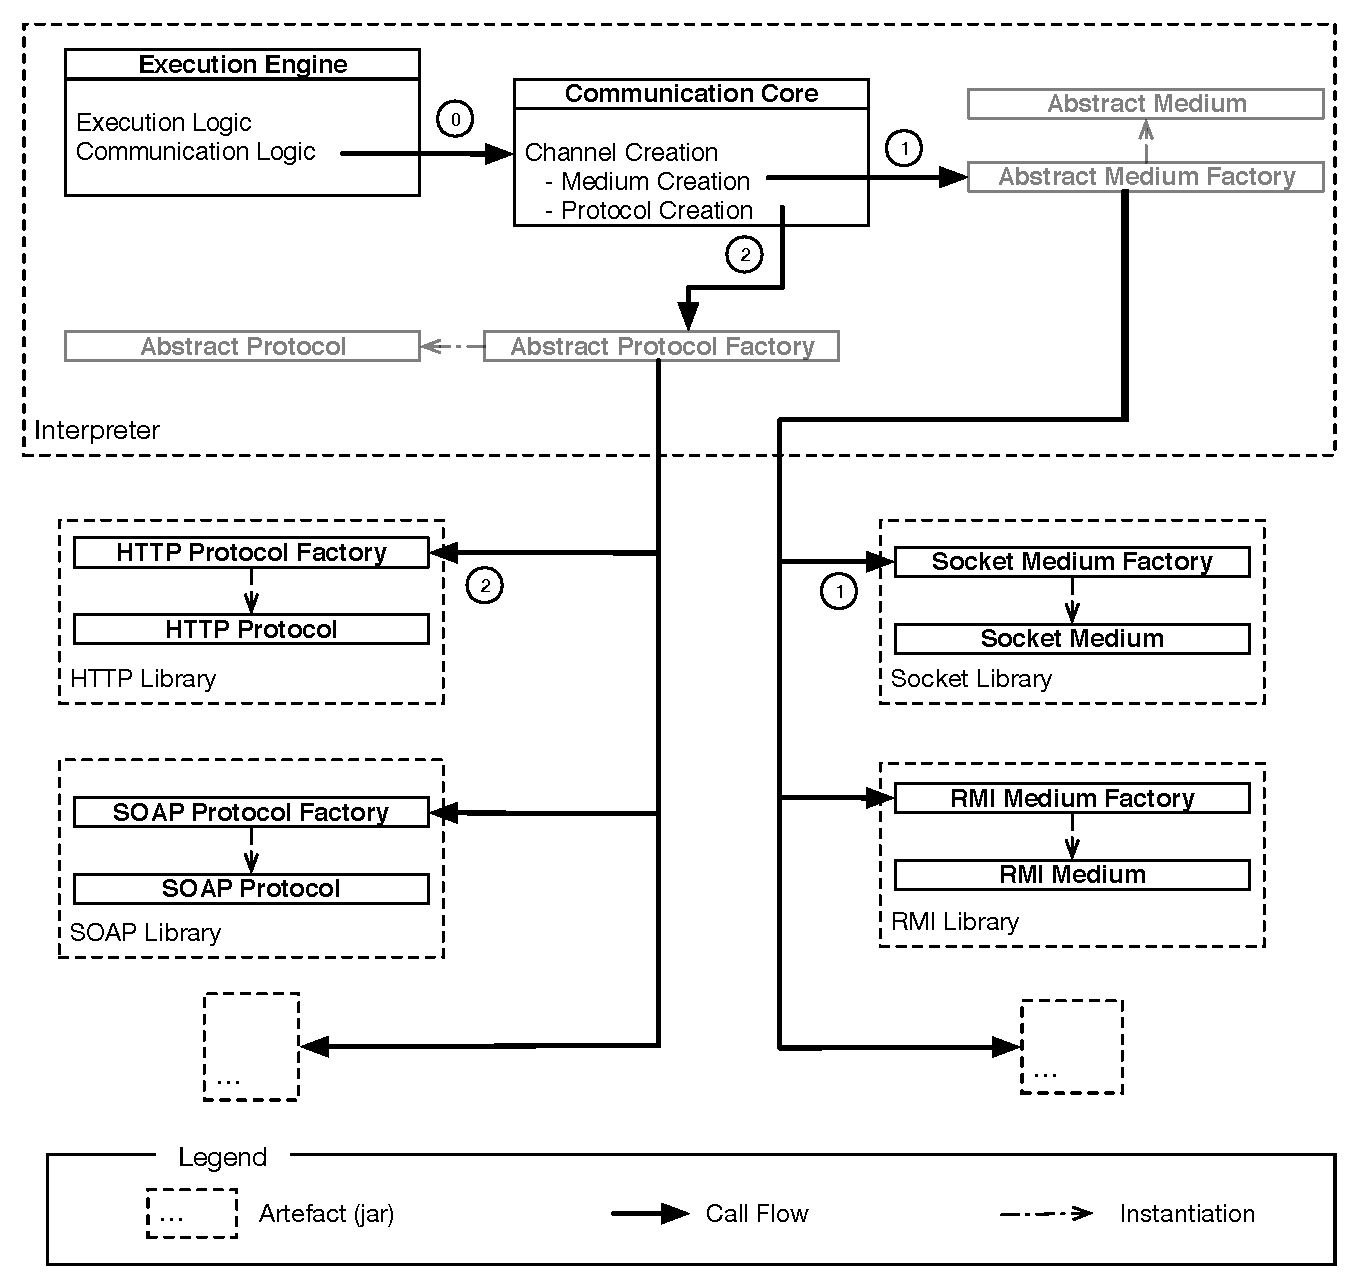
\includegraphics[width=\textwidth]{comm_modules.pdf}
  \caption{Conceptual representation of the call flow among the Jolie
  interpreter and its communication libraries.}
  \label{fig:comm_modules}
\end{figure}

\subsection{Implementation of CoAP/UDP in Jolie} % (fold)
\label{sec:impl_coap_udp}
%
Since by specification the CoAP protocol relies on the UDP medium protocol, in
order to integrate CoAP in Jolie we also had to integrate the UDP medium. As
described in \Cref{sub:jolie_extensions}, this entailed the creation of two
new libraries for the Jolie interpreter: a medium library for UDP and a
protocol library for CoAP.

We remark that, since UDP and CoAP are independent libraries, our
implementation of UDP can also be used to support other protocols relying on
UDP, such as MQTT-SN~\cite{hunkeler08}. The implementation of UDP consists in
a listener and a channel class, both based on the Netty
framework~\cite{maurer16}. Since the structure expected by Jolie and the one
provided by Netty are similar, the integration of UDP is smooth. An
interesting point is that exceptions raised by Netty are captured and
transformed into Jolie exceptions. These exceptions are notified to the
application protocol, which can either manage them or raise them at the level
of the behavior of the Jolie program.

The implementation of the CoAP library consists in a class taking care of encoding and decoding the message abstraction of Jolie, namely the Communication Message, into a CoAP formatted one. A second class, handling the encoding and decoding of a CoAP message into a buffer of bytes, is based on the work done in nCoAP~\cite{ncoap}, an open source project providing a CoAP implementation for Java, based itself on Netty.

We notice that CoAP supports request-response communications and, in 
particular, CoAP messages include fields \emph{i}) to specify 
at which address the reply is
expected and \emph{ii}) to match a reply with a previous request. Hence, the
implementation of \code{RequestResponse} communications in CoAP is sound also
with a transport protocol which is not connection-oriented, such as UDP.\@ This
would be a problem for protocols that do not provide such a facility, such as
HTTP, which is indeed not commonly used over UDP.

Notably, Jolie comes with a formal semantics (in terms of a process
calculus)~\cite{Guidi2006}, which enables to rigorously reason on the behavior
of Jolie programs. This has been instrumental in the evolution of the language,
e.g., to specify and prove properties on the fault handling mechanisms of the
language~\cite{GuidiLMZ09} or to correctly implement sessions~\cite{MontesiC11}
based on correlation mechanisms~\cite{bpel}. The semantics in~\cite{Guidi2006}
only considers reliable communications and needs to be extended to also cover
the unreliable case. We do not report here on this topic, since it is not
central for the purpose of this paper.

\subsection{Implementation of MQTT in Jolie.} % (fold)
\label{sub:impl_mqtt}

By specification, MQTT relies on the TCP/IP protocol, already implemented in
Jolie. This means that, theoretically, the implementation of MQTT would have
only entailed the creation of a dedicated MQTT protocol library. However, as
detailed in \Cref{sub:jolie_extensions}, Jolie assumes an end-to-end
communication pattern where the caller initiates the creation of a
communication channel with a server, which in turn expects such inbound
requests. For this reason, given a certain medium, \code{inputPort}s and
\code{outputPort}s use a medium-specific implementation of, respectively, a
listener class and a channel class.
%
This pattern, separating listeners from senders, does not apply to
publish/subscribe protocols, where both the subscriber and the publisher need
to establish a connection with the broker. In our implementation, we mediated
between the two approaches with a Publish-Subscribe medium, which is
essentially a wrapper implementing the logic of Publish-Subscribe message
handling on any other point-to-point medium available (TCP socket in the case
of MQTT) to the interpreter. Although we strove to separate the concerns
between the Jolie interpreter and this new Public-Subscribe channel, we had to
introduce a minimal update into the Jolie \textsf{Communication Core} so that it could
choose between the standard end-to-end media and the new wrapper.

The MQTT protocol class both encodes and decodes messages and implements the QoS
policies of the MQTT standard. Concretely, as for CoAP, we based the
implementation of MQTT on Netty~\cite{maurer16}. The main difficulty in the
implementation of the protocol is the definition of the message patterns needed
to implement \code{OneWay} and \code{RequestResponse} communications, which have
been described in \Cref{sub:mqtt}. Beyond being invoked when operations are executed, the
MQTT class is also invoked when the program is started, to perform port
initialization. In particular, this is when subscriptions to topics identified
in \code{inputPort}s are performed (along with the related connections to the
Brokers).


\section{Case Study}
\label{sub:case}
\begin{figure}[t]
  \centering
  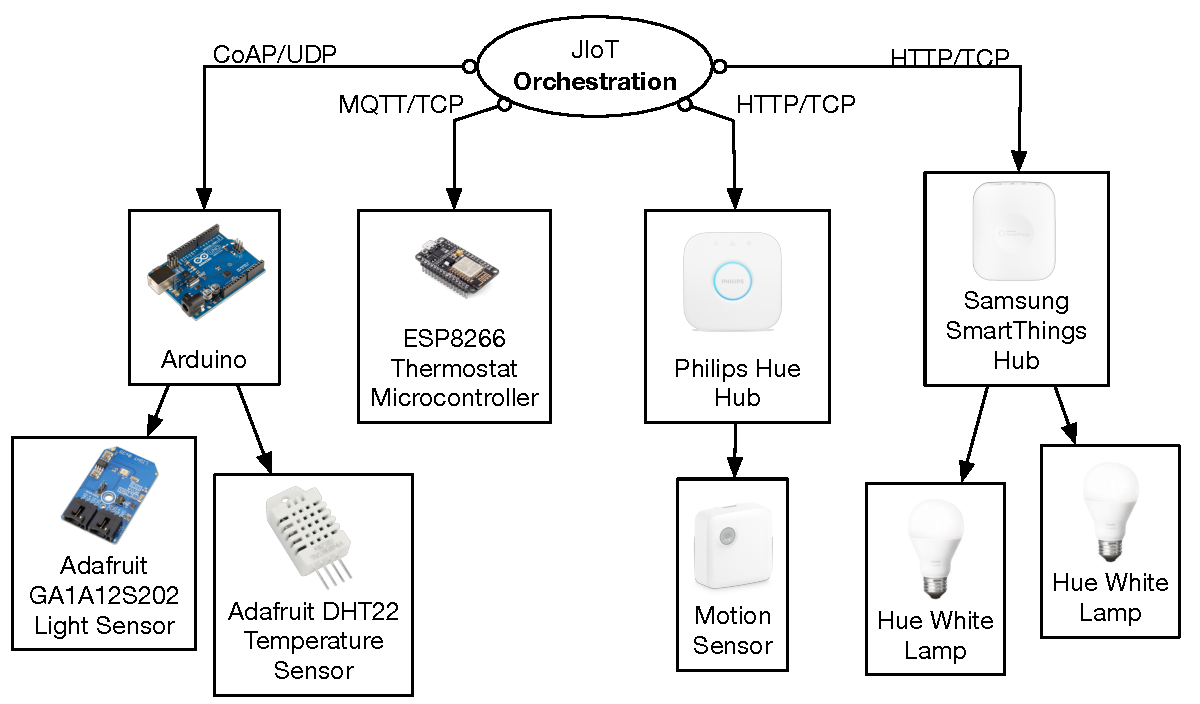
\includegraphics[width=\textwidth]{case_study_overview.pdf}
  \caption{Conceptual overview of the home automation case study.}
  \label{fig:case_study_overview} \end{figure}

In this section, we detail the programming of a home automation case study with
JIoT. We remark that the techniques presented in this case study are not
specific to home automation and can be used in any setting where heterogeneous
IoT technology stacks need interact. The use case is peculiar as new edge
devices can be included in the system at runtime. The source code of the system
is released under the GPL v.3 license and available at~\cite{jiot}. We report
in \cref{fig:case_study_overview} a schematic overview of the case study, where
Cloud nodes and mid-tier controllers (represented by the element labeled ``JIoT
Orchestration'' in \cref{fig:case_study_overview}) are programmed in JIoT and
orchestrate the behavior of a number of heterogeneous edge devices (whose
low-level programming is omitted here):

\begin{itemize} 

\item \emph{Philips Hue Hub}: a hub to control the Philips Hue smart home
devices;

\item \emph{Philips Hue White Lamps}: connected to the hub above; \item
\emph{Samsung SmartThings Hub}: a hub to control devices following  the
SmartThings specification~\cite{60};

\item \emph{Samsung SmartThings Motion Sensor}: connected to the hub above and
used as a presence sensor;

\item \emph{Arduino Uno}: a general-purpose microcontroller;

\item \emph{Adafruit GA1A12S202 Analog Light Sensor}: connected to the Arduino
above;

\item \emph{Adafruit DHT22 Temperature Sensor}: also connected to the Arduino
above;

\item \emph{ESP8266}: a microcontroller to manage a pre-existing  thermostat.

\end{itemize}

The case study combines commercial solutions --- e.g., the Philips Hue Hub and
the Hue White Lamps system where the Lamps are controlled by the Hub --- with
custom ones --- these span from sensors directly connected to a board, as it
happens for the Adafruit DHT22 temperature sensor, to solutions that integrate
a pre-existing hardware, like the ESP8266 that manages a pre-existing
thermostat. As illustrated in \cref{fig:case_study_overview}, this
heterogeneity of devices provides for a comprehensive scenario where we need
JIoT programs that use different application and transport protocols. In
particular, Philips and Samsung Hubs communicate with the orchestrator over
HTTP/TCP, the Arduino over MQTT/TCP, and the ESP8266 over CoAP/UDP.

In the use case we build a simple logic providing two functionalities: lighting
and temperature system control. The lighting system turns on the lights when
the motion sensor detects someone at home and the outdoor luminosity is below
some threshold. The temperature control checks the temperature and turns on the
heating system when the temperature is below some threshold. The threshold has
different values depending on whether someone is at home or not.

\begin{figure}[b]
  \centering
  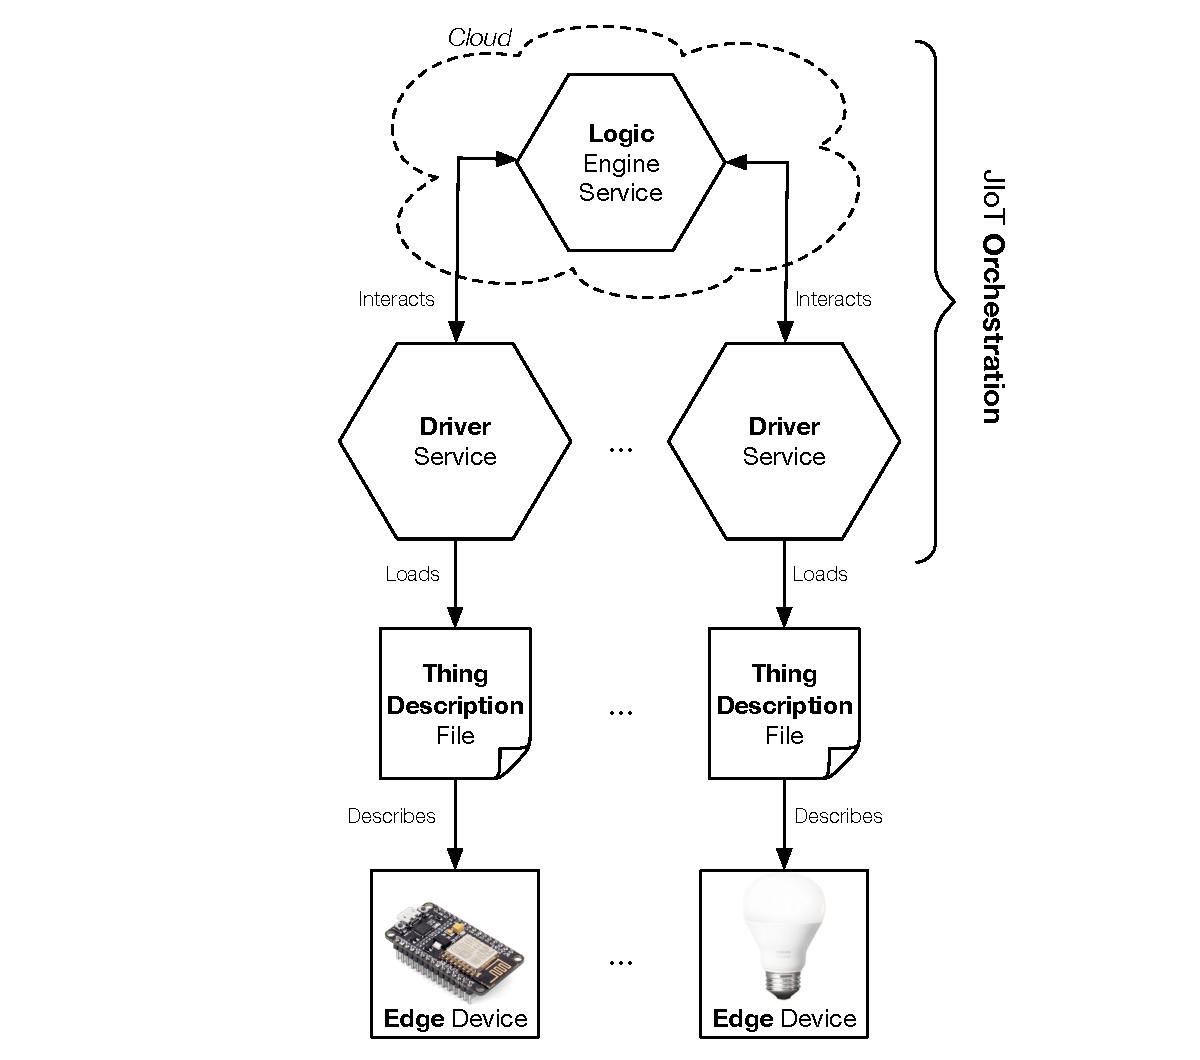
\includegraphics[width=.8\textwidth]{case_study_abstraction.pdf}
  \caption{Scheme of orchestration in the case study.}
  \label{fig:case_study_abstraction}
\end{figure}

\subsection{Structure of the Orchestration}

We now describe the structure of the orchestration in the case study, which is
illustrated in~\cref{fig:case_study_abstraction}.
%
The orchestration is composed of multiple JIoT programs. From top to bottom of
\cref{fig:case_study_abstraction}, the \texttt{LogicEngine} contains the general
logic of system control (i.e., the one that collects the data from sensors and
coordinates the execution of the actuators in the system). Since the
\texttt{LogicEngine} interacts with a multitude of mid-tier devices, its
natural deployment is in the Cloud, where it is possible to scale it according
to the number of managed devices and the load of computation. At the mid-tier
level we have JIoT \texttt{Driver}s. Each \texttt{Driver} interacts with a
specific edge device and it is deployed in a mid-tier machine in the proximity
of the controlled edge device.

\subsection{Thing Descriptors}

In the case study, the \texttt{Driver}s are statically configured to manage a
single fixed device using a JSON-LD 1.1 (that stands for JSON Linkage Data)
configuration file~\cite{jsonld}. The choice of JSON-LD is not mandatory, but
it has the benefit of following the standard W3C Web of Things~\cite{w3c17}
definition of Thing Description (TD). This makes our \texttt{Driver}s already
compliant with other WoT frameworks, simplifying future integrations with
other WoT systems.

While discussing the full structure of TD is out of the scope of this
paper, we present in \cref{fig:sensor_descriptor_1,fig:sensor_descriptor_2} examples of TDs used in our
case study. In \cref{fig:sensor_descriptor_1} we report the TD
for the DHT22 temperature sensor. For each device the JSON-LD file
specifies whether it is a sensor or an actuator (key \lstinline|"type"|) and
provides a textual description (key \lstinline|"description"|) and its name
(key \lstinline|"name"|). Each TD provides a list of
properties (key \lstinline|"properties"|) that can be read. Each property is
described by the property identifier, \lstinline{"temperature"} in our
example. The property identifier has various sub-elements describing it. In
our example we use just key \lstinline{"label"} to describe the unit of
measure.


\begin{figure}[b]
  \centering
  \begin{lstlisting}[language=json]
{
  "type": "sensor",
  "description": "Thing uses JSON-LD 1.1 serialization",
  "name": "Adafruit DHT22 Temperature Sensor",
  "properties": [
    {
      "temperature": {
        "label": "Celsius"
      }
    }
  ]
}
\end{lstlisting}
\caption{Adafruit DHT22 Thing Descriptor.}
  \label{fig:sensor_descriptor_1}
\end{figure}


\begin{figure}[tb]
\centering
\begin{lstlisting}[language=json]
{
  "type": "actuator",
  "description": "Thing uses JSON-LD 1.1 serialization",
  "name": "Philips Hue White Lamp",
  "actions": {
    "toggleLight": {
      "description": "Turn on or off the lamp."
    }
  }
}
\end{lstlisting}
  \caption{Philips Hue White Lamp Thing Descriptor.}
  \label{fig:sensor_descriptor_2}
\end{figure}

JSON-LD configuration files for MQTT and HTTP devices are similar. Also
configuration files for sensors and actuators are similar. As an example, we
report in \cref{fig:sensor_descriptor_2} the configuration file for Philips Hue
White Lamps. There the main differences with respect to the previous TD (\cref{fig:sensor_descriptor_1}) are:
%
\begin{itemize}
  
  \item the \lstinline{"type"} is now
  {\small\color{color:comment}\texttt{"actuator"}};

  \item the key \lstinline{"actions"} replaces the key
  \lstinline{"properties"};

  \item the key \lstinline{"description"} is used also to describe the single
  action.

\end{itemize}
%
In principle a TD can describe multiple properties belonging to a group of one
or more edge devices controlled by the same \texttt{Driver}. For simplicity,
here we have one TD for each edge device and, correspondingly, one
\texttt{Driver} that controls one edge device. We also assume that each sensor
provides one property.

\subsection{System Deployment}

Deployment-wise, JIoT provides a vast choice regarding what technology stack to
use between the \texttt{LogicEngine} and the \texttt{Driver}s.
%
Moreover, since both programs are developed in JIoT, it is easy to change their
deployment, switching to the technology stack that best suites a given scenario
(e.g., HTTP, to exploit caching, or binary formats like
SODEP~\cite{MontesiGZ14}, to limit bandwidth usage). Here, we choose to use the
HTTP/TCP stack to make our system compatible with many existing third-party
solutions --- currently HTTP/TCP is supported by the majority of software
systems~\cite{richardson2008restful}. However, different technology stacks fit
different purposes. The benefit of JIoT is that programmers can re-use the same
software components adapting their deployment to the desired communication
stacks. For example, if our goal was to be natively compatible with other
JavaScript IoT frameworks, we could have used the JSON-RPC binary protocol; if
we wanted to deploy our system as part of a Service-Oriented
Architecture~\cite{Erl07}, we could have used the SOAP protocol.

While JIoT-to-JIoT deployment is flexible, the deployment towards edge devices
is defined by the technology supported by the edge device. Concretely, in our
case study each \texttt{Driver} communicates with its edge device using (one
of) the protocol(s) supported by the latter.


\subsection{Components Behavior}

When started, a \code{Driver} loads the TD configuration file of its edge
device. Then it proceeds to register itself to the \code{LogicEngine}. In the
registration, it sends the information retrieved from the TD, enriched with two
additional pieces of information: the address where the edge device can be
contacted --- i.e., the \code{Driver} location --- and the identifier of the
user to which the edge device belongs. Once registered, the \code{Driver} acts
as a forwarder between the \code{LogicEngine} and the edge device.

The \code{LogicEngine} runs on the Cloud and manages a number of sensors and
actuators. More precisely the \code{LogicEngine} has one running session for
each user (distinguished according to the user identifier), managing all her
sensors and actuators. Each session is associated with an array of devices
that can be scanned to find the location of \code{device}s with particular
properties and interact with them. As an example, we report at lines 10--26 of
\Cref{lst:logic_example_get} the procedure \code{getTemperature} of the
\code{LogicEngine}, which computes the average temperature recorded by the
sensors of one user.
%
\begin{figure}[b]
\begin{lstlisting}[
basicstyle=\footnotesize\ttfamily,
label=lst:logic_example_get,
caption=\code{LogicEngine} \texttt{Driver} \code{outputPort} and \code{getTemperature} procedure.]
interface driverInterface {
  RequestResponse: engineRequest( request )( response )
}

outputPort Driver {
  Protocol: http
  Interfaces: driverInterface
}

define getTemperature {
 sum = 0 ;
 n = 0 ;
 for ( device in devices ) {
  if( device.<@\textcolor{black}{type}@> == "sensor" &&
    is_defined( device.properties.temperature ) ) {
   Driver.location = device.driverLocation ;
   request.operationName = "getTemperature" ;
   engineRequest@Driver( request )( response ) ;
   sum = sum + response.deviceResponse ;
   n++
  }
 } ;
 if( n!=0 ) {
  temperature = sum / n
 }
}
\end{lstlisting}
\end{figure}

\newpage

Briefly, procedure \code{getTemperature}:

\begin{itemize}
  \item scans the \lstinline{devices} structure (line 13) containing all
  registered \code{Driver}s;
  \item selects those whose {\small\texttt{type}} is \code{"sensor"} and have
  a property (under the sub-structure \code{properties}) named
  \lstinline{temperature}. Note how Jolie tree-shaped variables ease the
  exploration of structured data; in this case the one sent by the
  \code{Driver}s at registration time (and read from their associated JSON-LD
  file);
  \item it dynamically sets (line 16) the location of \code{outputPort Driver}
  (lines 5-8) to contact the selected \code{Driver};
  \item it sets the request operation to \code{getTemperature} (line 17);
  \item it retrieves the temperature sensed by the edge device controlled by
  the selected \code{Driver}, invoking it through operation
  \code{engineRequest};
  \item it aggregates the sensed temperature in variable \code{sum} and keeps
  track of the number of requests in variable \code{n} (lines 19--20);
  \item it computes the mean \code{temperature} (lines 23--25).
\end{itemize}
%

\begin{figure}[b]
\begin{lstlisting}[
basicstyle=\footnotesize\ttfamily,
label=lst:logic_example_set,
caption=\code{LogicEngine} setTemperature procedure.]
define setTemperature {
 for ( device in devices ) {
  if( device.<@\textcolor{black}{type}@> == "actuator" &&
    is_defined( device.properties.temperature ) ) {
   Driver.location = device.location ;
   request.operationName = "setTemperature" ;
   request.deviceRequest = comfortTemperature ;
   engineRequest@Driver( request )( response )
  }
 }
}
\end{lstlisting}
\end{figure}

The procedures that calculate the mean of the sensed external luminosity and
the one to check the presence of people at home are similar to the one in
\cref{lst:logic_example_get}, except that the searched properties are
\lstinline{light} in the first case, and \lstinline{motion} in the second.

We report in \cref{lst:logic_example_set} one of the procedures managing
the actuators, specifically the one used to set the temperature. The main
difference with respect to the logic in \cref{lst:logic_example_get} is that
procedure \code{setTemperature}:

\begin{itemize}
  \item selects the \lstinline{devices} whose {\small \texttt{type}} is
  \lstinline{"actuator"} (line 3);
  \item sets the request operation to \code{"setTemperature"} and passes the value
  in variable \code{comfortTemperature} as parameter of the request
  (lines 6-7).
\end{itemize}

Note that the operation called on the \code{Driver} is \code{engineRequest}
both in \cref{lst:logic_example_get} and \cref{lst:logic_example_set}. This
support the extension of the \code{LogicEngine} with new procedure definitions
that implement a given goal without requiring to change the interface between
the \code{LogicEngine} and the \code{Driver}s. In turn, a request with the same
\code{operationName} (e.g., \code{"setTemperature"}) triggers different
behaviors in different \code{Driver}s, as each implements the specific logic
of interaction with its associated edge device.
%

% They
% would register their devices one-by-one using a suitable security scheme
% (basic, token, api key, etc.). The selection of the security scheme can also
% be specified in the JSON-LD TD. Every time a device for a new user is
% registered, a session of the \code{LogicEngine} managing the devices owned by
% the user is spawned. Thus, new users and new devices can enter the system at
% any time.

\subsection{Cloud Deployment}

We conclude this section by describing the Cloud deployment of the
\code{LogicEngine}, which is containerized using
Docker~\cite{Merkel:2014:DLL:2600239.2600241}. The container is deployed
automatically into an Amazon Web Service cluster via the Docker Swarm
manager~\cite{Soppelsa:2017:NDC:3153103}. The \code{LogicEngine} is deployed in
the worker cluster, allowing the manager to balance the load of requests. We
report in \cref{lst:docker} the content of the Dockerfile used to deploy the \code{LogicEngine}.
%

\begin{figure}[b]
\begin{lstlisting}[
label=lst:docker,
caption=The Dockerfile used to deploy the \code{LogicEngine}.
]
<@\textcolor{red}{FROM}@> openjdk:alpine

<@\textcolor{red}{RUN}@>  java -jar jiot.jar -jh /usr/lib/jolie/ -jl /usr/bin/
<@\textcolor{red}{ENV}@> JOLIE_HOME /usr/local/lib/jolie

<@\textcolor{red}{ADD}@> logic_engine.ol /home/.
<@\textcolor{red}{WORKDIR}@> /home
<@\textcolor{red}{RUN}@> jolie logic_engine.ol
\end{lstlisting}
\end{figure}

%
At line 1 we declare the starting image for the container, which is the
lightweight Linux Alpine distribution with OpenJDK 8 pre-installed. At lines
3--4 we install the JIoT fork interpreter and we set the environmental
variable \code{JOLIE_HOME} to point to the location of the installed interpreter. At lines 6--7 we add the source code of the
\code{LogicEngine} in the home directory of the image.
Finally, at line 8 we start the execution of the \code{LogicEngine}.


\section{Related Work}
\label{sec:related}
In the literature there are many proposals for platforms, middlewares, smart
gateways, and general systems, all aimed at solving the interoperability
problem arising from the current ``babel'' of IoT technologies (protocols,
formats, and languages). Without any claim of being complete, here we mention a
few notable examples which are somehow related to the topic of the current paper.

Recently the W3C started the Web of Things (WoT) Working Group~\cite{w3c17}. The
aim of WoT is to define a standard stack of layered technologies, as well as
software architectural styles and programming patterns, to uniform and simplify
the creation of IoT applications. In this context, the W3C is working on a WoT
Architecture~\cite{wot.arch}. The main concept of the architecture is the notion
of ``servient'', a virtual entity that represents a physical IoT device.
Servients provide technology-independent, standard APIs that developers can use
to transparently operate in heterogeneous environments. Remarkably, both the
WoT proposal and ours concern high-level
abstractions for low-level access to devices provided via, e.g., HTTP, CoAP, and
MQTT.\@ However, while we propose a dedicated language, they provide API
specifications.
%
More in general, there are many proposals for the integration of WoT and IoT.\@
For example~\cite{dominique2011web} and~\cite{corredor2014lightweight} define
general platforms covering different layers of IoT, including an accessibility
layer which integrates concepts like smart gateways and proxies to facilitate
the connection of (smart) Things into the Internet infrastructure, using
architectural principles based on REST.
%
Smart gateways and proxies are used in several industrial proposals to
facilitate the development of applications. Common denominator of some of these
proposals, e.g.,~\cite{60,61,62}, is the abstraction of low-level
functionalities provided by embedded devices (e.g., connectivity and
communication over low-level protocols like ZigBee, Z-Wave, Wi/IP/UPnP, etc.).
Smart gateways are used also to translate (or integrate) CoAP into
HTTP~\cite{7811451,s150101217,7037719} and to integrate both CoAP and MQTT by
means of specific middlewares~\cite{6827678}. Eclipse IoT~\cite{EplicseIoT} is
an IoT integration framework proposed by the Eclipse IoT Working Group. Aim of
Eclipse IoT is to build an open IoT stack for Java, including the support for
device-to-device and device-to-server protocols, as well as the provision of
protocols, frameworks, and services for device management. There exist several
 European projects, notably INTER-IoT~\cite{7471373} and
symbIoTe~\cite{Gojmerac16}, that address the issue of interoperability in IoT
and have produced several concrete proposals. Finally, a work close to ours
is~\cite{Zhiliang11}, where a middleware converts IoT heterogeneous networks
into a single homogeneous network.

Although related to our aim in this paper, the cited proposals tackle the
problem of IoT integration from a framework perspective: they provide chains of
tools, each addressing a specific level of the integration stack. Differently,
we extend a language specifically tailored for system integration and advanced
flow manipulation, Jolie, to support integration of IoT devices. This offers a
single linguistic domain to seamlessly integrate disparate low-level IoT devices
and intermediate nodes (collectors, aggregators, gateways). Moreover, Jolie is
already successfully used for building Cloud-based, microservice
solutions~\cite{GabbrielliGGMM16,MelisPGC17}. This makes the language useful
also for assembling advanced architectures for IoT, e.g., to handle real-time
streaming and processing of data from many devices. The benefit, here, is that,
while solutions based on frameworks require dedicated proficiencies on each of
the included tools, Jolie programmers can directly work at any level of the IoT
stack, without the need to acquire specific knowledge on the tools in a given
framework.

To conclude our revision of related work, we narrow our focus on language-based
integration solutions for IoT. The work most related to ours is
SensorML~\cite{SensorML}.
%
SensorML, abbreviation of Sensor Model Language, is a modeling
language for the description of sensors and, more in general, of measurement
processes. Some features modeled by the language are: discovery and
geolocalization of sensors, processing of sensor observations, and
functionalities to program sensors and to subscribe to sensor events.
%
While some traits of SensorML are common to our proposal, the scopes of the two
languages sensibly differ. Indeed, while Jolie is a high-level language for
programming generic architectures (spanning from Cloud-based microservices to
low-level IoT integrators), SensorML just models IoT devices, their discovery,
and the processing of sensor observations.

%


\section{Discussion and Conclusion}
\label{conclusion}
In this paper, we proposed a language-based approach for the integration of
disparate IoT platforms. We built our treatment on the Jolie programming
language. This first result is an initial step towards a more comprehensive
solution for IoT ecosystem integration and management. Concretely, we included
in Jolie the support for two of the most widely used IoT protocols. The
inclusion enables Jolie programmers to interact with the majority of present IoT
devices. Summarizing our results: \emph{i}) we included in Jolie the CoAP
application protocol, also extending the Jolie language to support the UDP
transport protocol, \emph{ii}) we added the support for the MQTT protocol and,
in doing so, \emph{iii}) we tackled the challenging problem of mapping the
renowned pattern of request-responses (typical of HTTP and other widely used
protocols) into the publish/subscribe message pattern of MQTT.\@ The mapping
abstracts from peculiarities of MQTT and is applicable to any publish/subscribe
protocol.

Regarding future work, we are currently investigating the integration in Jolie
of more IoT protocols~\cite{7123563}, in order to extend the usability of the
language in the IoT setting.

It would also be interesting to extend not only the Jolie interpreter, as we
have done, but also the formal model behind
it~\cite{Guidi2006,MontesiC11,GiallorenzoMG18}. To this end, we can take ideas
from the formal model of IoT systems presented in~\cite{LaneseBF13}.

%%%%%%%%%%%%%%%
%Another interesting direction comes from the inclusion of publish/subscribe
%protocols in Jolie. Indeed, the publish/subscribe pattern is renowned for
%enabling high scalability of networks, as well as supporting flexible and highly
%dynamic network topologies~\cite{eugster03}. Our intuition is that, besides
%efficiency and scalability, publish/subscribe architectures can achieve a higher
%degree of reliability if programmed using the Jolie language.
%%%%%%%%%%%%%%%
% Moreover, the
% communication abstractions provided by the language avoid the use of callbacks,
% which are difficult to program, debug, and are one of the main causes of errors
% in concurrent and distributed systems~\cite{fukuda15}.

Another interesting direction for future developments is studying how Jolie
can support the testing of IoT technologies, e.g., to test how
different protocol stacks perform over a given IoT topology. Thanks to the
simplicity of changing the combination of the used protocols (application and
transport), experimenters can quickly test many configurations, also enjoying
a more reliable platform to compare them. Indeed, usually even changing one
of the protocols in the configured stack would require an almost complete
rewrite of the logic of network components. Contrarily, in Jolie, this change
just requires an update of the deployment part of programs, leaving the logic
unaffected. Moreover, such an update could even be done programmatically,
making the practice of repeated experimenting on IoT networks easier and more
standardized.

Finally, as future work, we also consider the possibility of developing a
light-weight version of the language, to be used on low-power IoT devices.
Indeed, in this paper, we assumed that these devices are programmed with
low-level languages, since they can support only a very constrained execution
environment. Clearly, letting programmers develop all the components of an IoT
network in the same language would not only ease its implementation but also
testability, deployment, and maintenance. However, achieving such a result
would require a very challenging engineering endeavor.


\subsubsection*{Acknowledgments} % (fold)
We thank Marco Di Felice, Luca Bedogni, and Federico Montori for useful
suggestions and comments.

% section section_name (end)

% \vspace{5em}

\bibliographystyle{ieeetr}
{\bibliography{biblio}}

\end{document}
